\documentclass[11pt,a4paper]{article}

\usepackage[margin=1in]{geometry}
\usepackage{booktabs}
\usepackage{enumitem}
\usepackage{hyperref}
\usepackage{amsmath}
\usepackage{float}
\usepackage{setspace}
\usepackage{tikz} 
\usetikzlibrary{shapes.geometric, arrows.meta, positioning}

\setstretch{1.15} 

\title{\textbf{ML-Based Flood Prediction System Using Historical Threat Mapping and Live Weather APIs}}

\author{
    \textbf{Submitted to: Dr. Jeelani} \\[0.5cm]
    Amit Bishnoi (1024240005) \\
    Diksha Garg (1024240015) \\[0.5cm]
    Thapar Institute of Engineering and Technology
}
\date{August 2026}

\begin{document}

\maketitle

\section{Introduction \& Problem Statement}
Floods cause massive damage around the world. Because of climate change, they are happening more often, making it crucial to have better ways to predict them. Right now, weather apps show us live data like rain and wind, but they do not tell us if that rain will actually cause a flood in a specific area. 

On the other hand, traditional flood maps are usually drawn once and rarely updated. They cannot react to a sudden, heavy storm. Also, databases that track past disasters (like EM-DAT) have great details on the damage caused, but they often lack exact GPS coordinates. Because of this, current systems struggle to instantly connect a live storm with a location's history of flooding.

Our project aims to fix this gap. We are building a system that takes live weather data and compares it against a combined database of past floods. By merging the exact GPS data from the Dartmouth Flood Observatory (DFO) with the impact records from EM-DAT, our machine learning model will be able to predict the real-time flood risk for any searched location.

\section{Literature Review}
Past flood prediction relied heavily on complex physical models of rivers and terrain, which require immense computing power and are difficult to scale for smaller cities. While Machine Learning (ML) has emerged as a faster alternative to predict water levels, current systems largely fail to integrate live weather API data with long-term disaster records. This project bridges that gap by treating geographic vulnerability as dynamic, mixing real-time weather conditions with historical data to calculate an instant, automated risk score.

\section{Objectives}
The main goal of this project is to build a machine learning system that uses live weather data and past disaster records to predict current flood risks.

Specific steps to achieve this include:
\begin{itemize}[noitemsep]
    \item To pull real-time weather data (like rainfall, temperature, and wind speed) using the OpenWeatherMap API.
    \item To clean and combine the EM-DAT and DFO datasets to create a complete history of floods with exact GPS coordinates.
    \item To create custom data features for our model, such as past flood severity and how much it rained in the last 48 hours.
    \item To train and test machine learning models to predict if the flood risk is Low, Medium, or High.
    \item To build a simple user interface where anyone can search a location and see its live weather and risk score.
\end{itemize}

\section{Methodology \& System Architecture}
The project relies on a five-stage data pipeline, taking raw live signals and turning them into a final risk score. The overall system architecture is illustrated in Figure \ref{fig:architecture}.

\begin{figure}[H]
    \centering
    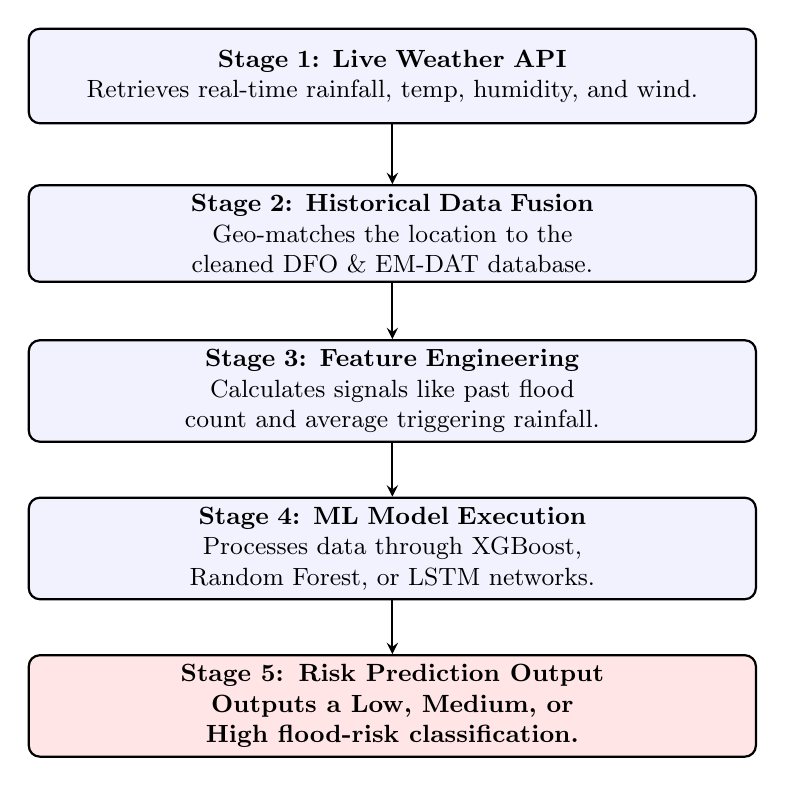
\begin{tikzpicture}[
        node distance=2cm,
        stageBlock/.style={
            rectangle, rounded corners, draw=black, thick,
            fill=blue!5, text width=9cm, text centered, minimum height=1.2cm,
            font=\small
        },
        finalBlock/.style={
            rectangle, rounded corners, draw=black, thick,
            fill=red!10, text width=9cm, text centered, minimum height=1.2cm,
            font=\small\bfseries
        },
        arrow/.style={
            thick, ->, >=stealth
        }
    ]
        % Nodes
        \node (stage1) [stageBlock] {\textbf{Stage 1: Live Weather API} \\ Retrieves real-time rainfall, temp, humidity, and wind.};
        \node (stage2) [stageBlock, below of=stage1] {\textbf{Stage 2: Historical Data Fusion} \\ Geo-matches the location to the cleaned DFO \& EM-DAT database.};
        \node (stage3) [stageBlock, below of=stage2] {\textbf{Stage 3: Feature Engineering} \\ Calculates signals like past flood count and average triggering rainfall.};
        \node (stage4) [stageBlock, below of=stage3] {\textbf{Stage 4: ML Model Execution} \\ Processes data through XGBoost, Random Forest, or LSTM networks.};
        \node (stage5) [finalBlock, below of=stage4] {\textbf{Stage 5: Risk Prediction Output} \\ Outputs a Low, Medium, or High flood-risk classification.};

        % Arrows
        \draw [arrow] (stage1) -- (stage2);
        \draw [arrow] (stage2) -- (stage3);
        \draw [arrow] (stage3) -- (stage4);
        \draw [arrow] (stage4) -- (stage5);
    \end{tikzpicture}
    \caption{System Architecture: A five-stage data pipeline, from live signal to risk score.}
    \label{fig:architecture}
\end{figure}

\subsection{Stage 1: Live Weather API}
The system starts by searching a specific location. It pulls real-time rainfall, temperature, humidity, and wind speed for that exact spot using a live weather API (OpenWeatherMap).

\subsection{Stage 2: Historical Data}
Next, the system looks at the past. We clean and filter historical flood events using our merged DFO and EM-DAT database, geo-matching those past events to the user's searched location based on exact coordinates.

\subsection{Stage 3: Feature Engineering}
In this stage, we take the raw data and derive useful signals for the AI to understand. This includes calculating metrics like the past-flood count for that area and the average flood rainfall it usually takes to trigger a disaster there.

\subsection{Stage 4: ML Model Training}
The processed data is then fed into our machine learning models so the system can learn the risk patterns. We have two main model options for this stage:
\begin{itemize}[noitemsep]
    \item \textbf{XGBoost / Random Forest:} These are best for tabular data and will output a simple Low, Medium, or High classification.
    \item \textbf{LSTM Networks:} These are best for tracking multi-day weather trends, allowing for true time-series forecasting.
\end{itemize}

\subsection{Stage 5: Risk Prediction Output}
Finally, the system fuses all this information and outputs a clear, easy-to-understand Low, Medium, or High flood-risk score for the user on the front-end interface.

\section{Evaluation Criteria}
To make sure our model actually works, we will test it using 20\% of our historical data that the model has not seen before. We will measure its success using:
\begin{itemize}[noitemsep]
    \item \textbf{Precision, Recall, and F1-Score:} This helps us balance false alarms with missed warnings.
    \item \textbf{ROC-AUC:} This checks how well the model can separate Low, Medium, and High risk levels.
    \item \textbf{Speed:} The system should show the final risk score in under 2 seconds after the user searches a location.
\end{itemize}

\section{Project Timeline}
\begin{table}[H]
\centering
\begin{tabular}{@{} l p{7.5cm} p{5cm} @{}}
\toprule
\textbf{Phase} & \textbf{Task Description} & \textbf{Key Deliverable} \\ \midrule
Weeks 1--3 & Read existing research, set up API keys, and clean the data. & Cleaned dataset \& working API code \\
Weeks 4--7 & Combine DFO and EM-DAT data, and start training ML models. & Trained models \& accuracy reports \\
Weeks 8--10 & Connect the backend code to the front-end user interface. & Working software prototype \\
Weeks 11--12 & Fix bugs, improve the design, and write the final report. & Final project file \& presentation \\ \bottomrule
\end{tabular}
\end{table}

\section{Resources \& Risk Assessment}
\subsection{Resources Needed}
We will use free, open-source Python libraries (like Scikit-Learn and Pandas) and public datasets (EM-DAT and DFO). The live weather data will come from the free version of the OpenWeatherMap API. We will use our own laptops for coding and training the models, so the project requires zero budget.

\subsection{Possible Risks \& Solutions}
\begin{itemize}
    \item \textbf{Mismatched Data:} When combining EM-DAT and DFO, some dates or locations might not match perfectly. \textit{Solution:} We will write code that matches events that happened within a few days of each other, rather than looking for exact date matches.
    \item \textbf{Imbalanced Data:} The dataset will naturally have more "safe" days than "flood" days, which can confuse the model. \textit{Solution:} We will use a technique called SMOTE to balance the training data so the model learns fairly.
    \item \textbf{API Limits:} Free weather APIs only let you make a limited number of requests per day. \textit{Solution:} We will save (cache) our recent searches so we do not have to keep calling the API for the same location while we are testing the code.
\end{itemize}

\section{Summary}
This project proposes a deployable, machine learning-driven platform to reduce flood-related damages by providing instant, localized risk assessments. By successfully fusing high-resolution spatial data with historical impact metrics and live weather APIs, it overcomes the severe limitations of traditional, static flood maps. The system is designed to be accessible, cost-effective, and highly scalable, offering a vital early warning tool for both everyday users and emergency responders.

\end{document}